\section{Q-Band Suppression Theory}

\subsection{Reduced Roll-Sloshing Excitation Model}
Oneline Full liquid state prediction requires observation from liquid\cite{Komasa2023observing}, which is not always available. To avoid full state prediction, a reduced model is established to explain why only band suppression from input is enough for anti-rollover and how to identify dangerous frequency components. The unsprung lateral motion is represented by a lateral cart, the sprung mass by a roll pendulum, and the dominant liquid mode by a pendulum attached to the tank body. Taken lateral acceleration $a_y$ as input, the coupled roll-sloshing dynamics can be linearized as
\begin{equation}
    \mathbf{M}\ddot{\mathbf{x}}_r+\mathbf{C}\dot{\mathbf{x}}_r+\mathbf{K}\mathbf{x}_r=\mathbf{B}_a \ay ,~\mathbf{x}_r=[\phi,\theta,\dot{\phi},\dot{\theta}]^\T ,
    \label{eq:reduced_roll_slosh}
\end{equation}
where $\phi$ is the tank-body roll angle and $\theta$ is the relative liquid sloshing angle. The off-diagonal terms in $\mathbf{M}$ and $\mathbf{K}$ describe the coupled free mode between suspension roll and liquid motion as
\begin{equation}
\det(\mathbf{K}-\omega^2\mathbf{M})=0 .
\end{equation}
Therefore, the dangerous frequency is not the isolated liquid natural frequency or the roll frequency, they appeal to each other and generate a broad-peak.

\begin{figure}[!t]
\centering
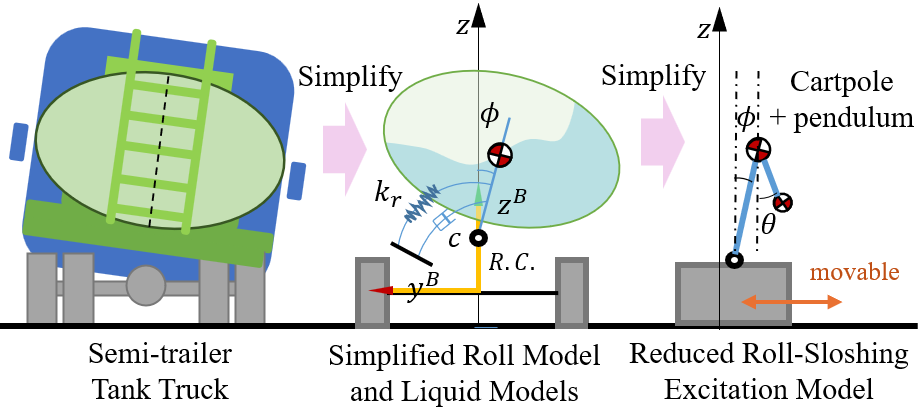
\includegraphics[width=\linewidth]{fig/reduced_roll_sloshing_model.png}
\caption{Reduced lateral model. The online controller only needs the frequency response between input and output.}
\label{fig:simplified_model}
\end{figure}


\subsection{Critical Band and Risk Bound}
Let the rollover-risk output be
\begin{equation}
    z=C_z\mathbf{x}_r+D_z\ay ,
\end{equation}
where $z$ represents LTR, roll angle, or another rollover indeces, and in this work the roll rate is used as the measurable risk-output. From \eqref{eq:reduced_roll_slosh}, the input-output frequency response is
\begin{equation}
    G_{za}(s)=C_z(s^2\mathbf{M}+s\mathbf{C}+\mathbf{K})^{-1}\mathbf{B}_a+D_z .
    \label{eq:freq_response}
\end{equation}
The Q-band $\mathcal{B}_i=[f_i^-,f_i^+]$ is selected around the broad-peak region of $|G_{za}(j2\pi f)|$. In this work the main band is centered on the dominant sloshing-related response, with additional bands covering secondary and higher-frequency coupled excitations.

Safety could be stated as a sufficient frequency-domain condition. Let $a_{y,\mathcal{B}}$ denote the lateral-acceleration component in a target band $\mathcal{B}$, and let $z_{\mathcal{B}}$ be the corresponding risk-output component. Around the calibrated operating point, assume that the linearized system is stable and
\begin{equation}
    |G_{za}(j2\pi f)|\leq \bar{G}_{\mathcal{B}},\qquad f\in\mathcal{B}.
\end{equation}
Then Parseval's relation gives
\begin{equation}
    \|z_{\mathcal{B}}\|_2^2
    \leq \bar{G}_{\mathcal{B}}^2\|a_{y,\mathcal{B}}\|_2^2 .
    \label{eq:qband_parseval}
\end{equation}
Thus, if $\|a_{y,\mathcal{B}}\|_2^2\leq\bar E_{\mathcal{B}}$, where $\bar E_{\mathcal{B}}$ is the given band-energy threshold,
\begin{equation}
    \|z_{\mathcal{B}}\|_2 \leq \bar{G}_{\mathcal{B}}\sqrt{\bar E_{\mathcal{B}}}.
    \label{eq:qband_sufficient_bound}
\end{equation}
Considering static load-transfer contribution and bounded residual terms, a conservative rollover margin can be written as
\begin{equation}
    |\LTR_{\mathrm{stat}}|+\bar{G}_{\mathcal{B}}\sqrt{\bar E_{\mathcal{B}}}
    +R_\perp+R_0+R_m\leq \LTR_{\mathrm{lim}},
    \label{eq:ltr_margin_condition}
\end{equation}
where $R_\perp$, $R_0$, and $R_m$ bound non-target-band excitation, initial roll/slosh energy, and model or sensing errors, respectively.
\textit{Proof:} Inequality \eqref{eq:qband_parseval} follows from the frequency-domain gain bound of the stable linearized input-output model. Substituting the band-energy threshold gives \eqref{eq:qband_sufficient_bound}. Adding the bounded static, off-band, initial-condition, and model-error contributions yields \eqref{eq:ltr_margin_condition}. The condition is sufficient rather than necessary, and its conservatism comes from linearization, band discretization, gain upper bounding, and residual margins.

This proof explains why limiting the band energy of $\ay$ can reduce rollover-risk excitation even when liquid phase and true wheel loads are not observed online. The discrete Q-band matrix used by the controller is an implementable approximation of $\|a_{y,\mathcal{B}}\|_2^2$ over the prediction horizon.

% % TODO（作者）：最终稿需要给出由扫频、TruckSim 或模型车辨识得到的危险频带。当前 MATLAB 脚本采用 0.35--0.75 Hz 作为主频带，并覆盖 0.75--1.45 Hz 等次级频段；后续应写清楚这些频段的标定来源和对应的 \bar E_i 阈值。

% \subsection{Online and Offline Quantities}
% The online Q-band controller depends on predicted lateral acceleration, vehicle speed, steering state, yaw response, and reference preview. Liquid angle, true wheel loads, and high-fidelity LTR are not required online. They are used offline to calibrate dangerous bands and to evaluate simulation or model-truck safety. This separation is important for trailer-sensing-limited deployment.
